\documentclass[11pt,a4paper]{article}
\usepackage[a4paper, top=1.5cm, bottom=1.5cm]{geometry}
\usepackage{musicography}
\usepackage{tikz}
\usepackage{atbegshi}

% Credits

\AtBeginShipoutNext{\AtBeginShipoutUpperLeft{%
  \put(15,-\paperheight + 15){%
    \parbox[b][\paperheight]{\paperwidth}{%
      \vfill
      {\tiny See also: https://www.youtube.com/watch?v=PEcWZUnOUEY (Stichmethod)}
    }%
  }%
}}

% End of Credits

% Remove pagenumbering
\pagestyle{empty}

% Define the \dash command -> " - "
\newcommand{\dash}{\hspace{0.4em}-\hspace{0.4em}}

\begin{document}

% Chromatic Scale section
\begin{center}
\textbf{CHROMATIC SCALE}
\end{center}

\begin{center}
A{\dash}A\musSharp/B\musFlat{\dash}B{\dash}C{\dash}C\musSharp/D\musFlat{\dash}D{\dash}D\musSharp/E\musFlat{\dash}E{\dash}F{\dash}F\musSharp/G\musFlat{\dash}G{\dash}G\musSharp/A\musFlat
\end{center}
% End of Chromatic Scale section

\vspace{0.5cm}

% Major scale formula
\begin{center}
\textbf{MAJOR SCALE FORMULA}
\end{center}

\vspace{-0.4cm}

\begin{table}[h]
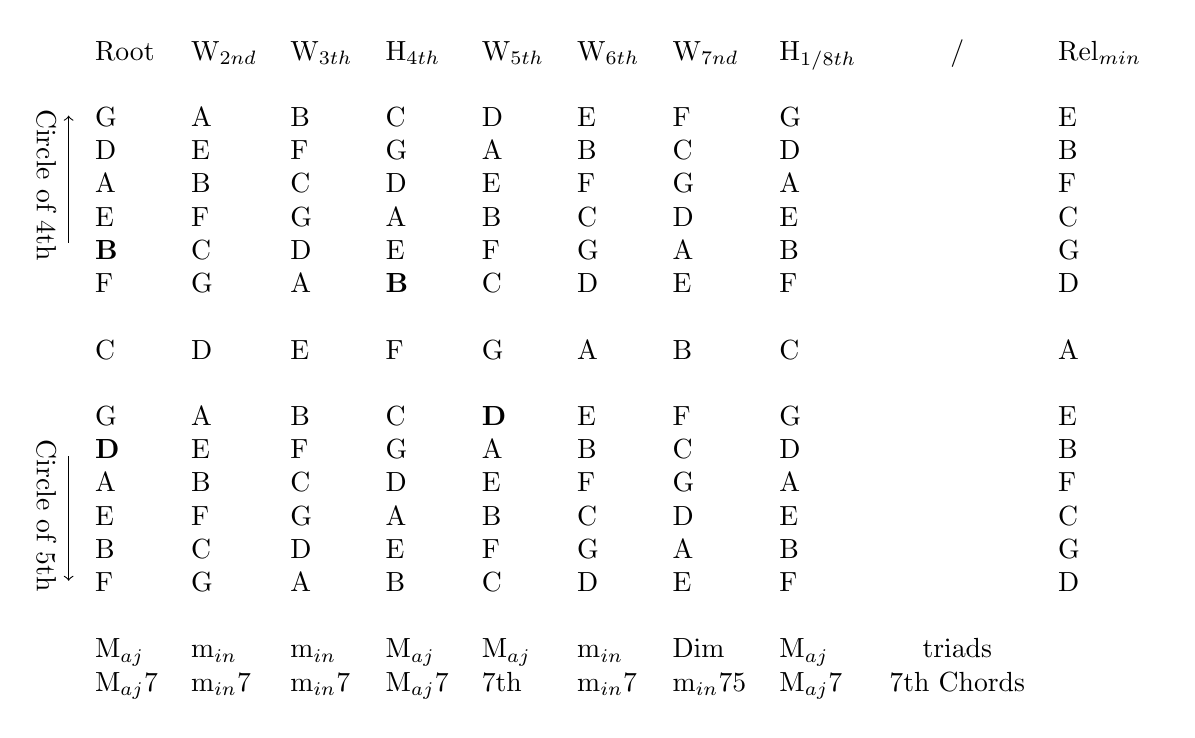
\begin{tikzpicture}
  \node (table) {
	\begin{tabular}{l l l l l l l l c l}
		Root & W$_{2nd}$ & W$_{3th}$ & H$_{4th}$ & W$_{5th}$ & W$_{6th}$ & W$_{7nd}$ & H$_{1/8th}$ & \musSharp/\musFlat & Rel$_{min}$ \\
		\\
		G\musFlat & A\musFlat & B\musFlat & C\musFlat & D\musFlat & E\musFlat & F & G\musFlat & \musFlat\musFlat\musFlat\musFlat\musFlat\musFlat & E\musFlat \\
		D\musFlat & E\musFlat & F & G\musFlat & A\musFlat & B\musFlat & C & D\musFlat & \musFlat\musFlat\musFlat\musFlat\musFlat & B\musFlat \\
		A\musFlat & B\musFlat & C & D\musFlat & E\musFlat & F & G & A\musFlat & \musFlat\musFlat\musFlat\musFlat & F \\
		E\musFlat & F & G & A\musFlat & B\musFlat & C & D & E\musFlat & \musFlat\musFlat\musFlat & C\\
		\textbf{B\musFlat} & C & D & E\musFlat & F & G & A & B\musFlat & \musFlat\musFlat & G \\
		F & G & A & \textbf{B\musFlat} & C & D & E & F & \musFlat & D \\
		\\
		C & D & E & F & G & A & B & C & & A \\
		\\
		G & A & B & C & \textbf{D} & E & F\musSharp & G & \musSharp & E\\
		\textbf{D} & E & F\musSharp & G & A & B & C\musSharp & D & \musSharp\musSharp & B\\
		A & B & C\musSharp & D & E & F\musSharp & G\musSharp & A & \musSharp\musSharp\musSharp & F\musSharp \\
		E & F\musSharp & G\musSharp & A & B & C\musSharp & D\musSharp & E & \musSharp\musSharp\musSharp\musSharp & C\musSharp \\
		B & C\musSharp & D\musSharp & E & F\musSharp & G\musSharp & A\musSharp & B & \musSharp\musSharp\musSharp\musSharp\musSharp & G\musSharp \\
		F\musSharp & G\musSharp & A\musSharp & B & C\musSharp & D\musSharp & E\musSharp & F\musSharp & \musSharp\musSharp\musSharp\musSharp\musSharp\musSharp & D\musSharp \\
		\\
		M$_{aj}$ & m$_{in}$ & m$_{in}$ & M$_{aj}$ & M$_{aj}$ & m$_{in}$ & Dim & M$_{aj}$ & triads \\
		M$_{aj}$7 & m$_{in}$7 & m$_{in}$7 & M$_{aj}$7 & 7th & m$_{in}$7 & m$_{in}$7\musFlat5 & M$_{aj}$7 & 7th Chords \\
		\end{tabular}
	};
	\draw [->] ([shift={(0pt,-155pt)}]table.north west) -- ([shift={(0pt,47pt)}]table.south west) node[midway, above, sloped, xshift=-1pt, yshift=-15pt]{Circle of 5th};
	\draw [<-] ([shift={(0pt,-32pt)}]table.north west) -- ([shift={(0pt,169pt)}]table.south west) node[midway, above, sloped, xshift=2pt, yshift=-15pt]{Circle of 4th};
\end{tikzpicture}
\end{table}
% End of Major scale formula

% Minor scale formula
\begin{center}
\textbf{MINOR SCALE FORMULA}
\end{center}

\vspace{-0.4cm}

\begin{table}[h]
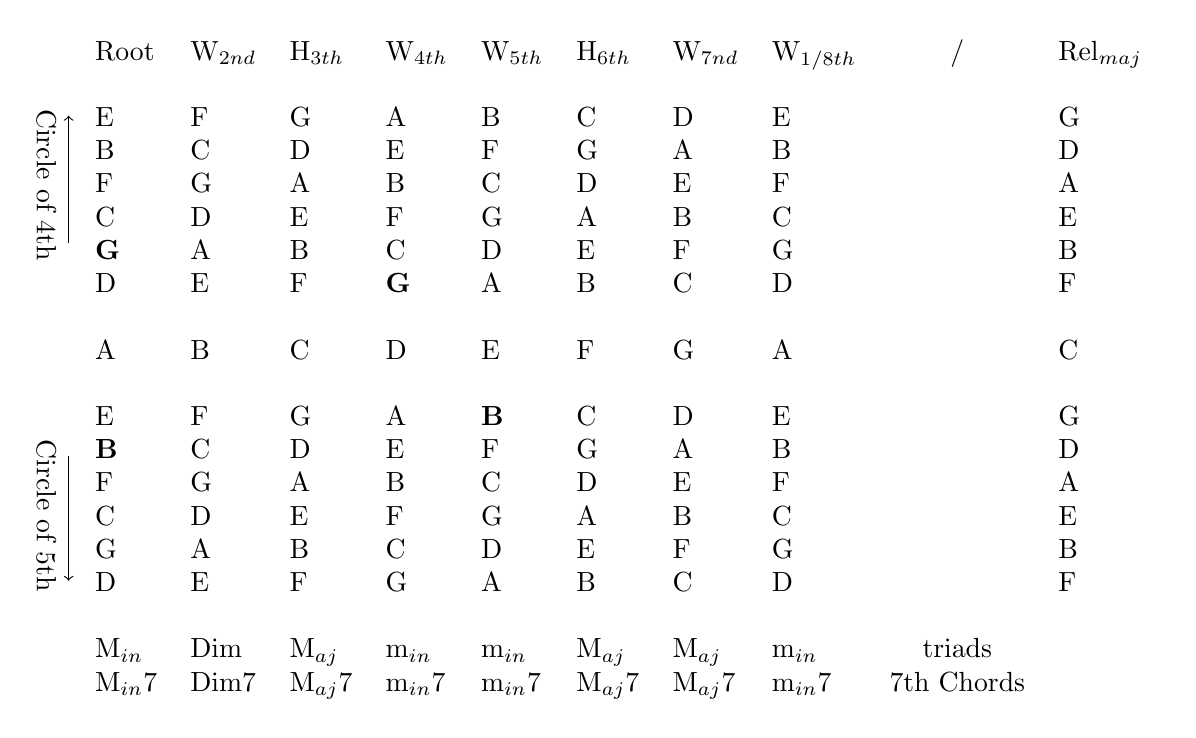
\begin{tikzpicture}
  \node (table) {
	\begin{tabular}{l l l l l l l l c l}
		Root & W$_{2nd}$ & H$_{3th}$ & W$_{4th}$ & W$_{5th}$ & H$_{6th}$ & W$_{7nd}$ & W$_{1/8th}$ & \musSharp/\musFlat & Rel$_{maj}$ \\
		\\
		E\musFlat & F & G\musFlat & A\musFlat & B\musFlat & C\musFlat & D\musFlat & E\musFlat & \musFlat\musFlat\musFlat\musFlat\musFlat\musFlat & G\musFlat\\
		B\musFlat & C & D\musFlat & E\musFlat & F & G\musFlat & A\musFlat & B\musFlat & \musFlat\musFlat\musFlat\musFlat\musFlat & D\musFlat \\
		F & G & A\musFlat & B\musFlat & C & D\musFlat & E\musFlat & F & \musFlat\musFlat\musFlat\musFlat & A\musFlat \\
		C & D & E\musFlat & F & G & A\musFlat & B\musFlat & C & \musFlat\musFlat\musFlat & E\musFlat\\
		\textbf{G} & A & B\musFlat & C & D & E\musFlat & F & G & \musFlat\musFlat & B\musFlat\\
		D & E & F & \textbf{G} & A & B\musFlat & C & D & \musFlat & F \\
		\\
		A & B & C & D & E & F & G & A &  & C \\
		\\
		E & F\musSharp & G & A & \textbf{B} & C & D & E & \musSharp & G \\
		\textbf{B} & C\musSharp & D & E & F\musSharp & G & A & B & \musSharp\musSharp & D \\
		F\musSharp & G\musSharp & A & B & C\musSharp & D & E & F\musSharp & \musSharp\musSharp\musSharp & A \\
		C\musSharp & D\musSharp & E & F\musSharp & G\musSharp & A & B & C\musSharp & \musSharp\musSharp\musSharp\musSharp & E \\
		G\musSharp & A\musSharp & B & C\musSharp & D\musSharp & E & F\musSharp & G\musSharp & \musSharp\musSharp\musSharp\musSharp\musSharp & B \\
		D\musSharp & E\musSharp & F\musSharp & G\musSharp & A\musSharp & B & C\musSharp & D\musSharp & \musSharp\musSharp\musSharp\musSharp\musSharp\musSharp & F\musSharp \\
		\\
		M$_{in}$ & Dim & M$_{aj}$ & m$_{in}$ & m$_{in}$ & M$_{aj}$ & M$_{aj}$ & m$_{in}$ & triads \\
		M$_{in}$7 & Dim7 & M$_{aj}$7 & m$_{in}$7 & m$_{in}$7 & M$_{aj}$7 & M$_{aj}$7 & m$_{in}$7 & 7th Chords \\
		\end{tabular}
	};
	\draw [->] ([shift={(0pt,-155pt)}]table.north west) -- ([shift={(0pt,47pt)}]table.south west) node[midway, above, sloped, xshift=-1pt, yshift=-15pt]{Circle of 5th};
	\draw [<-] ([shift={(0pt,-32pt)}]table.north west) -- ([shift={(0pt,169pt)}]table.south west) node[midway, above, sloped, xshift=2pt, yshift=-15pt]{Circle of 4th};
\end{tikzpicture}
\end{table}
% End of Minor scale formula


% Notes
\noindent \textbf{Note:} When borrowing chord from another scale, always use the adjacent scale. E.g. If the root$_{maj}$ is A\musFlat\hspace{0.1cm}you can use chords from the key of D\musFlat\hspace{0.1cm}or E\musFlat
% End of Notes

\vfill
\end{document}